\section{La détection de communauté}
\subsection{Motivations}
La théorie des réseaux, a pour but d'analyser les graphes correspondant à des réseaux tels que celui de l'Internet, de la politique ou de la classification en biologie.
Chacun de ces graphes ont des propriétés spécifiques telles que:
\begin{itemize}
 	\item[-] \underline{Centrality}: mesure de cohésion du graphe ;
 	\item[-] \underline{``small world effect''}:  distance moyenne entre deux nœuds est proportionnelle au log du nombre de nœuds dans le graphe;
 	\item[-] \underline{Clustering}: mesure du regroupement des nœuds du graphe;
 	\item[-] \underline{Efficiency}: mesure la résistance du graphe;
 	\item[-] \underline{Degree distribution}; 
 	\item[-] \underline{Community Structure}.\\
 \end{itemize}
C'est cette dernière propriété qui va nous intéresser, à savoir la structure de communauté d'un graphe.
L'idée de communauté correspond à l'intuition selon laquelle il y a des nœuds qui ont un lien étroit et forment des sous ensembles de nœuds de ce graphe.
Par exemple dans le graphe des représentants politique Français, les hommes politiques d'un même partie appartiendraient à une même communauté.
Cependant, dans cet exemple les choses peuvent être plus subtiles que ça, c'est là qu'intervient la détection de communauté.

\subsection{Méthodes}
Il y a différentes classes de méthodes pour la détection de communauté, en voici une liste non exhaustive:
\begin{itemize}
	\item[-] Hierarchical clustering
	\item[-] Graph partitioning
	\item[-] Partitional clustering
	\item[-] Spectral clustering \\
\end{itemize}

\subsection{Comparaison des structures de communauté}
La notion de structure de communauté dans un graphe n'a pas de définition claire et consensuelle.
En effet, lorsque l'on veut faire de la détection de communauté nous cherchons d'hypothétiques lien entre les nœuds d'un réseau.
Cependant, ce lien ne peut pas avoir de sens a priori. 
Dans l'exemple du graphe du personnel politique français, si on trouve une certaine structure de communauté, quel sens peut-on donner au fait que deux personnes appartiennent à la même communauté.
Pour trouver un sens aux liens extraits par les algorithmes, on peut essayer de partir du sens de l'information à partir de laquelle le graphe a été construit, mais cela reste de l'ordre de l’interprétation.  

De plus, le résultat obtenu dépend entièrement du choix de la méthode utilisée.
La non unicité des résultats des algorithmes de détection de communauté rajoute une variabilité substantielle à l’interprétation d'une structure de communauté.
En substance, cela veut dire qu'en plus de choisir comment construire le graphe (i.e à partir de quelle information), il faut aussi choisir une métrique qui mesure la notion de proximité entre deux éléments du réseau.\\

Une conséquence négative de la non unicité des résultats est le fait qu'il n'existe pas de référence à partir de laquelle comparer les différentes structures de communautés obtenues.
Le seul moyen de juger le véracité des résultats obtenus est de les comparer entre eux et de faire une synthèse.
Il existe une abondante littérature sur la comparaison des méthodes.

On peut cependant essayer de comparer théoriquement les méthodes utilisés en analysant des graphes que l'on génère de manière aléatoire et dont on connaît les communautés.
On appelle ces graphes, ``graphe aléatoire'' ou `random graph'
Cette manière de procéder à l'avantage de posséder une référence à partir de laquelle comparer les algorithmes.
En revanche, les graphes générés ainsi ne correspondent pas forcement au graphes que l'on trouve dans la ``nature''.
Par conséquent des algorithmes qui ont de très bonnes performances sur un certain type de graphe, ne seront pas forcement pertinents sur des graphes générées à partir de données réelles. 

Une grande part de la recherche dans ce domaine est de rajouter des propriétés et des contraintes aux algorithmes de génération de graphes afin qu'ils satisfassent au mieux les propriétés des graphes que l'on observe dans la réalité (réseaux sociaux ...).
On peut donc ainsi trouver le meilleur algorithme pour un ensemble de graphes satisfaisant un certain nombre de propriétés.\\

Pour comparer les résultat a partir d'un graphe aléatoire il faut choisir une métrique.
Il existe une très grand nombre de métrique qui donnent là aussi des résultats divergeant.
On ne sait pas jusqu'à présent quel algorithme est le plus fiable.

Dans le cas où l'on utilise un graphe aléatoire, il existe plusieurs moyens de comparer les partitions obtenues avec la partition de référence.  
Pour une liste fournies des méthodes existante voir \cite[p.77-79]{Community_detection_in_graphs}.
Ci-dessous une liste non exhaustive des métriques qui seront utilisées ultérieurement.
\begin{itemize}
	\item[-] Fraction of correctly classified vertices ; 
	\item[-] Fowlkes and Mallows metric; 
	\item[-] Rand Index; 
	\item[-] Normalized Mutal Information; 
\end{itemize}

\subsection{Comparaison des performances}
Une autre problématique des algorithmes de détection de communautés est la performance.
En effet, beaucoup de méthodes considérées comme les plus efficaces du point de vue des communautés obtenues ont une complexité polynomiale voire exponentielle.
Or beaucoup de réseaux de vrai-monde ont un nombre de nœuds d'un ordre largement supérieur au milliard. 
On se retrouve donc dans le trade-off classique entre la performance et l'erreur d'approximation. 
Dans ces situations, il faut dont trouver des algorithmes à la fois performants et consistants.\\

C'est dans cette perspective que se place les papiers que nous étudions dans ce mémoire.
Nous nous placerons toujours dans le contexte d'un Stochastic Block Model, ou SBM, à 2 communautés de même taille et à deux probabilités $p_{in}$ et $p_{out}$.

Un SBM est un graphe aléatoire dans lequel on choisi un nombre de nœuds $n$, le nombre de communautés $q$. 
On génère ainsi une graphe à n nœuds sans arrêtes, et ensuite pour chaque pair de nœuds on simule une variable de Bernoulli pour décider si l’arrête existe ou non.
Le paramètre de la loi de Bernoulli est $p_{in}$ si les deux nœuds appartiennent à la même communauté et $p_{out}$ sinon.

Dans ce contexte, d'après le paragraphe \cite[Numerical results]{Spectral_Detection_in_the_Censored_Block_Model}, l'algorithme ``belief propagation'' est réputé pour être optimal sur les partitions rendues.
Ainsi, pour comparer les performances des algorithmes dans ce contexte, la littérature utilise cet algorithme comme un benchmark du point de vue de la répartition obtenue.
Ensuite ils comparent la performance et le temps d’exécution par rapport à celui-ci.
Ci-dessous une figure provenant de \cite{Spectral_redemption_clustering_sparse_networks} qui synthétise ce paragraphe.
\begin{figure}[H]
\centering
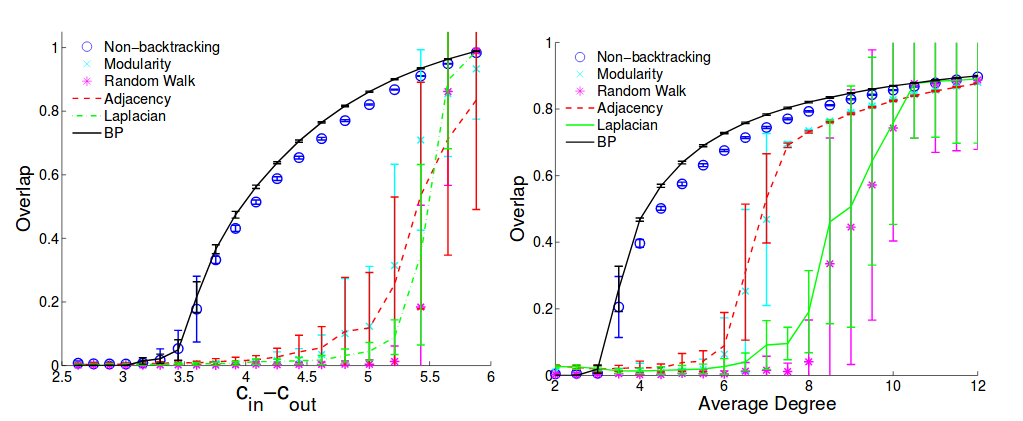
\includegraphics[scale=0.5]{static/bp_perf.png}
\caption{Précision des algorithmes de détection spectral basées sur différents opérateurs linéaires par rapport l'algorithme ``belief propagation''}
\end{figure}

\subsection{Perspectives}
Les limites des modèles spectraux qui sont en développement pour la détection de communauté sont les suivantes:
\begin{itemize}
	\item[1-] Seuil à partir duquel la méthode spectrale n'est plus en mesure de détecter le communauté ;  
	\item[2-] Temps de calcul sur de grands graphes;  
	\item[3-] Raffinement des modèles de communautés.  
\end{itemize}